%!TEX root = ../draft.tex
\chapter{Methodik und Durchführung}\label{s.methudurchf}
In diesem Kapitel werden die verwendeten Datensätze aufgeführt und die Umsetzung der Normalisierungsalgorithmen beschrieben.  
 \section{Vortrainierte Netze}\label{s.modell}
Das Unternehmen COCO \cite{common2018data} (Common Objects in Contexts) stellt eine Vielzahl an Datensätzen bereit mit denen neuronale Netze trainiert werden können. Bei den Datensäzen handelt es sich um unterschiedliche Objekte in verschiedenen Umgebungen.  
Einige Netze welchem mit dem COCO datensätzen traniert wurden stehen als \textit{Open Source} zur Verfügung. Die folgende Tabelle \ref{tab:cocomodels} führt ausgewählte neuronale Netze auf, um die Genauigkeit und Geschwindigkeit vergleichen zu können, damit ein geeignetes Netz für die Versuche ausgewählt werden kann.
\begin{table}
[h]
\caption{Künstliche neuronale Netze \cite{google2018tens} welche mit dem COCO Dataset Trainiert wurden \cite{common2018data}} 
\label{tab:cocomodels}
\centering
\begin{tabular}{|l|c|c|}
\hline
Neuronales Netz & mAP & Geschwindigkeit\\
\hline
faster\_rcnn\_inception\_v2\_coco & 28 & 58\\
faster\_rcnn\_resnet50\_coco & 30 & 89\\
rfcn\_resnet101\_coco & 30 & 92\\
ssd\_mobilenet\_v1\_coco & 30 & 21\\
ssd\_resnet\_50\_fpn\_coco & 35 & 76\\
\hline
\end{tabular}
\end{table}
Um die Auswirkungen der Normalisierung deutlich hervorheben zu können wurde bei der Auswahl des Netzes eins ausgewählt, welches eine recht niedrige mAP hat. \\
Das faster\_rcnn\_inception\_v2\_coco soll für das Projekt verwendet werden. Dieses hat eine \textit{mAP} von 28 und eine Geschwindigkeit von 32 ms. Dadurch das es die niedrigste \textit{mAP} hat, sollten die Auswirkungen, der Normalisierungsverfahren, in der Genauigkeit stärker ersichtlich werden. Das ausgewählte Netz wird im folgenden auf die Datensätze, welche im anschließenden Unterkapitel aufgeführt sind.
  \section{Trainingsdaten}\label{s.tdaten}
Da für ein solches Training die benötigten Trainingsdaten und die Zeit nicht zur Verfügung stehen, sollte eine Möglichkeit gefunden werden, wie das Training auch mit weniger Trainingsdaten durchgeführt werden kann. Durch das vortrainieren der neuronalen Netze, werden nur noch durchschnittlich 150 Bilder pro Objektklasse und eine geringere Trainingszeit benötigt. Die Bilder der eigenen Daten werden mit einer 13 Megapixel Kamera eines \textit{Huawei P Smart} aufgenommen. Die verwendeten Objekte werden von vielen verschiedenen Seiten aufgenommen. Dabei müssen für das Training, pro klasse ungefähr 150 Bilder vorhanden sein. Da die Bilder mit einer der Kamera mehrere Megabyte groß werden, müssen diese auf 100-300 KB komprimiert werden.\\
Damit am Ende des Projektes möglichst gute Vergleichswerte entstehen, werden mehrere Datensätze vor den Versuch verwendet. Insgesamt werden die neuronalen Netze mit 3 unterschiedlichen Datensätzen trainiert. Dafür wurden 3 Datensätze heraus gesucht. Der erste Datensatz welcher getestet wird, ist der Nahrungsmittel Datensatz eines früheren Projektes, zum anderen der Datensatz von \textit{Pascal Visual Object Classes} (PascalVOC) und der Hunderassen Datensatz, Stanford Dog Dataset.\\
In den folgenden Tabellen werden alle Datensätze mit den zugehörigen Klassen und Anzahl an Trainingsbildern aufgeführt:\\\\
Der erste Datensatz besteht aus mehreren Nahrungsmitteln, welche in der Tabelle \ref{tab:nahrungsmittel} jede klasse besitzt um die 100-150 Bilder welche zusätzlich Annotations-Dateien mit den Koordinaten der Klassifizierungsboxen (Kapitel \ref{s.trainingsdaten}) beinhalten. Dieser Datensatz ist mit seinen ca. 1000 Bildern der kleinste Datensatz. 
\begin{table}
[h]
\caption{Datensatz mit Nahrungsmitteln}
\centering
\begin{tabular}{|l|l|}
\hline
Klassenname & Klassenname\\
\hline
Milch - Packung & Orangensaft - Packung\\
Wasser - Flasche & Bier - Flasche\\
Brunch - Aufstrich & Margarine - Aufstrich\\
\hline
\end{tabular}
\label{tab:nahrungsmittel}
\end{table}
Der PascalVOC Datensatz umfasst 20 Klassen und besteht aus 5.000 Bildern. Von 2005 bis 2012 wurde jährlich die PascalVOC Challenges durchgeführt. Dabei sollte das beste verfahren für die Segmentierung, Klassifikation und Objekterkennung ermittelt werden. Inhaltlich befasst sich der Datensatz mit einer reihe unterschiedlicher Klassen, welche in Tabelle \ref{tab:pvoc} zu erkennen sind. Es gibt einige Unterschiede in der Häufigkeit der auftretenden Klassen. Beispielsweise sind in rund 2000 Bildern insgesamt 4.690 Personen enthalten, weswegen es möglicherweise Unterschiede in der Genauigkeit untereinander, der Klassen geben könnte. Die Aufnahmen der Bilder sind thematisch und und von der Art der Aufnahme unstrukturiert, was bedeutet, dass teilweise Bilder von einzelnen Objekten, Gruppen von Objekten oder auch ganze Szenen enthalten sind.
\begin{table}
[h]
\caption{Pascal Visual Object Classes \cite{pascal-voc-2007}}
\centering
\begin{tabular}{|l|l|l|l|}
\hline
Klassenname & Klassenname & Klassenname & Klassenname\\
\hline
Person & Vogel & Katze & Kuh\\
Hund & Pferd & Schaf & Zug\\
Flugzeug & Fahrrad & Boot & Bus\\
Auto & Motorrad & Flasche & Stuhl\\
Tisch & Blumentopf & Sofa & Bildschirm\\
\hline
\end{tabular}
\label{tab:pvoc}
\end{table}
Der dritte Datensatz welcher in dieser Arbeit verwendet wird, ist der Hunde Datensatz aus Stanford und beinhaltet 120 verschiedene Hunderassen. Jede Klasse hat um die 200 Bilddaten. Wegen der Struktur des Datensatzes, in einzelnen Ordnern, kann eine Auswahl der priorisierten Hunderassen zusammengestellt werden. Für den Versuch und damit eine bessere Übersicht erreicht werden kann, wurden 20 Hunderassen ausgewählt. Die Anotationen der Daten sind in Form von XML Dateien beigefügt. In der Tabelle \ref{tab:sdd} werden die ausgewählten Klassen des Datensatzes zusammengefasst.
\begin{table}
[h]
\caption{Stanford Dog Dataset \cite{KhoslaYaoJayadevaprakashFeiFei_FGVC2011}}
\label{tab:sdd}
\centering
\begin{tabular}{|l|l|l|l|}
\hline
Klassenname & Klassenname & Klassenname & Klassenname\\
\hline
Chihuahua & Japanese Spaniel & Maltese Dog & Pekinese\\
Shih-Tzu & Blenheim Spaniel & Papillon & Toy Terrier\\
Rhodesian Ridgeback & Afghan Hound & Basset & Beagle\\
Bloodhound & Bluetick & Coonhound & Walker Hound\\
Redbone & Borzoi & Irish Wolfhound & Italian Greyhound\\
\hline
\end{tabular}
\end{table}
Von der Struktur der Datensätze, sind sie ähnlich aufgebaut. Viele verschiedene Klassen mit verschiedenen Szenen und Kontexten. Im weiteren wird zunächst auf die Umsetzung der Normalisierungsverfahren eingegangen, um weiter Erkenntnisse zu erlangen.
\section{Normalisierung-Algorithmen}\label{s.nalgorithmen}
Für die Normalisierung der Datensätze ist eine Methode nötig, um mehrere Bilder möglichst schnell hintereinander zu bearbeiten. Für die Normalisierung wurden Python Programme geschrieben, welche nacheinander die Bilder, anhand eines Algorithmus verarbeitet. Dafür wurde mit unter die \textit{Python Image Libary} und OpenCV genutzt. Beide Bibliotheken werden für das verarbeiten von Bildern benötigt. 
\subsection{Gray-World-Algorithmus}
\begin{lstlisting}
# Importieren des Bildes
nimg = cv.imread(i, 1)
# Umwandlung des Bildes und der Kanäle in 32 Bit
nimg = nimg.transpose(2, 0, 1).astype(np.uint32)
# Zwischenspeichern des durchschnittlichen Grünkanals
mu_g = np.average(nimg[1])
# Berechnng des rot-Kanals: 
nimg[0] = np.minimum(nimg[0]*(mu_g/np.average(nimg[0])),255)
# Berechnung des blau-Kanals:
nimg[2] = np.minimum(nimg[2]*(mu_g/np.average(nimg[2])),255)
Zurükwandlung des Bildes in 8 Bit
img_output = nimg.transpose(1, 2, 0).astype(np.uint8)
\end{lstlisting}
Der Gray World Algorithmus \cite{gray2012world} welcher verwendet wird, funktioniert etwas anders als in den Grundlagen beschrieben. Für die Normalisierung der Kanäle, wird der durchschnitt des Grünkanal verwendet, da diese Farbe wichtig für das Helligkeitsempfinden ist. Das Bild wird zunächst in 32 Bit umgewandelt. Daraufhin wird  der Durchschnittswert des Grünkanals berechnet und zwischengespeichert. Der Grün-Kanal wird nun mit dem durchschnitt des Rot-Kanals dividiert und anschließend mit dem Minimum des Rot-Kanals multipliziert und übernommen. Der gleiche Vorgang folgt mit dem Blau-Kanal. Das verarbeitete Bild wird nun wieder zurück in 8 Bit gewandelt und ausgegeben (Abbildung \ref{img:gwnimg}). Für das verfahren wird keine spezielle Python Bibliothek eingesetzt.
\begin{figure}
	[h]
	\centering
	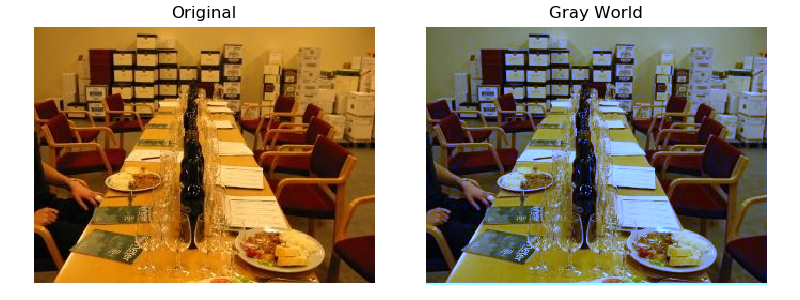
\includegraphics[scale=0.6]{Sources/gwn.png}
	\caption{Auswirkung des Gray-World Algorithmus}
	\label{img:gwnimg}
\end{figure}
\subsubsection{Histogramm Ausgleich}
\begin{lstlisting}
# Importieren des Bildes
img = cv2.imread('input.jpg')
# Umwandlung des Farbraumes von BGR zu YUV
img_yuv = cv2.cvtColor(img, cv2.COLOR_BGR2YUV)
# Ausgleichung vom Histogramm des Y Kanals
img_yuv[:,:,0] = cv2.equalizeHist(img_yuv[:,:,0])
# Umwandlung des Farbraumes in den BGR Farbraum
img_output = cv2.cvtColor(img_yuv, cv2.COLOR_YUV2BGR)
\end{lstlisting}
Für die Histogramm Ausgleichung \cite{histogram2012equalisation} wird das Bild zunächst vom BGR Farbraum in den YUV Farbraum (Kapitel \ref{s.lab} umgewandelt. Der Y-Kanal wird für die Histogramm Ausgleichung verwendet. Das hat den Grund, dass das Luminanzsignal oder auch Leuchtdichte-Signal die Summe der drei Grundfarben Rot Grün und Blau und die Helligkeitsinformation enthält. Das Histogramm des Y Kanals wird, wie in Kapitel \ref{s.histogramme} beschrieben, ausgeglichen. Das normalisierte Bild wird von dem YUV Farbraum zurück in den BGR Farbraum konvertiert und zwischengespeichert. Das Ergebnis wird als Bild ausgegeben (Abbildung \ref{img:histogrameq}).
\begin{figure}
	[h]
	\centering
	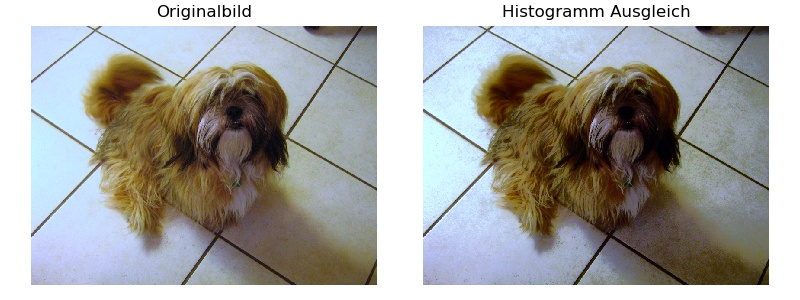
\includegraphics[scale=0.7]{Sources/histeq.jpg}
	\caption{Auswirkung der Histogramm Ausgleichung}
	\label{img:histogrameq}
\end{figure}	
\subsection{Histogramm Spezifikation}
\begin{lstlisting}
# Importieren des Referenzbildes
reference = io.imread('reference.jpg')
# Importieren des zu Normalisierenden Bildes
image = io.imread('image.jpg')
# Weiterleitung der beiden Bilder an die match_histogram-Methode der Skimage Bibliothek
matched = match_histograms(image, reference, multichannel=True)
\end{lstlisting}
Der dritte Normalisierungsfunktion welche für die Datensätze angewendet wird, ist die Histogramm Spezifikation (Kapitel \ref{s.hs}) oder auch \textit{Histogramm Matching}. Für den Algorithmus wird die Python Bibliothek \textit{Scikit-image} verwendet. Dafür werden ein Referenzbild und ein Zielbild geladen. Diese beiden Bilder, werden mit der Funktion \textit{match\_histograms} verarbeitet. Das Zielbild wurde auf das Histogramm des Referenzbildes angepasst. In dem Beispiel \ref{img:histogramspez} kann man gut erkennen, das das Quellbild, welches stark verdunkelt ist, durch ein gut ausgeleuchtetes Referenzbild, eine wesentlich bessere Helligkeit aufweist (Abbildung \ref{img:histogramspez}). Die Problematik bei dieser Normalisierungs Methode besteht darin, das ein einheitliches Referenzbild genutzt werden muss auf welchem dann der gesamte Datensatz Normalisiert wird.
\begin{figure}
	[h]
	\centering
	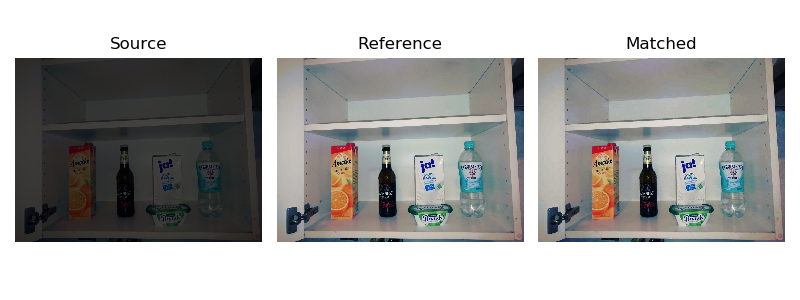
\includegraphics[scale=0.6]{Sources/HS_beispiel.png}
	\caption{Das Zielbild wurde mithilfe des Referenzbildes ausgeglichen und angepasst. Auf der linken Seite ist das Ergebnis der Spezifikation}
	\label{img:histogramspez}
\end{figure}